In~\cite[]{visser1997gravitational} Visser sets up a semi-analytical model in order to compute some contractions of the renormalized stress energy tensor for scalar fields non-minimally coupled to the Schwarzschild background metric, averaged on the Unruh vacuum.

We are again using the Unruh vacuum - as in~\cite[]{levi2016versatile} - which is the appropriate state to describe black hole evaporation, but we wish to expand the domain of validity of such result to non minimally coupled scalar fields, which are the ones we have been treating in the analysis of \(\mathcal{V}\), in subsection~\ref{subsec:non-min-EKG-theory}.

Moreover, a semi-analytical computation can allow us to understand the robustness of our result, which is what we are eventually interested in.

For the \((3 + 1)\) Unruh vacuum, it doesn't exist yet any analytic approximate expression for the stress energy tensor, and hence the need of a numerical approach. Visser's - and hence our - results are obtained using the Jensen-McLaughlin-Ottewill numerical data for the spin \(0\) Unruh vacuuum~\cite[]{jensen1991renormalized}. By spherical symmetry, for any \(s\)-wave quantum state \(\vert \psi\rangle\) 
\begin{equation}
    \label{eq:stress-tensor-s-wave}
    \langle\psi\vert T^{\mu\nu}\vert\psi\rangle = \begin{pmatrix}
        \rho & f & 0 & 0 \\
        f & -\tau & 0 & 0 \\
        0 & 0 & p & 0 \\
        0 & 0 & 0 & p
    \end{pmatrix}
\end{equation}

Here \(\rho\), \(f\), \(p\) and  \(\tau\) are functions of the radial coordinate \(r\), the mass of the black hole \(M\) and \(\hbar\), and we have set \(G = 1\); for later convenience \eqref{eq:stress-tensor-s-wave} is to be thought valid in the coordinate system \(\{t, r^*, \theta, \phi\}\), even if naturally the form of the tensor shall be the same in all the other coordinate system that do not mix angular coordinates with radial or time ones. We will refer to \(\{t, r, \theta, \phi\}\) as spherical coordinates, where the metric is espressed by the well-known expression:
\[
ds^2 =  \left(1 - \frac{R_s}{r}\right)dt^2  - \frac{dr^2}{1 - \frac{R_s}{r}} - r^2d\Omega^2,
\]
while \(r^*\) is the standard \emph{Tortoise} coordinate
\[
r^* \coloneqq r + R_s\ln\left(\frac{r}{R_s} - 1\right).    
\]

For compactness of notation we shall define \(z \coloneqq \frac{R_s}{r}\), where \(R_s = 2M\) is the Schwarzschild radius.
Visser relies on the decomposition of the stress energy tensor into \(4\) separately conserved quantities (in the Schwarzschild spacetime), as was shown in~\cite[]{christensen1977trace}: 
\[
    \langle\psi\vert T^{\mu\nu}\vert\psi\rangle = \left[T_{trace}\right]^{\mu\nu} + \left[T_{pressure}\right]^{\mu\nu} +
    \left[T_{+}\right]^{\mu\nu} + \left[T_{-}\right]^{\mu\nu}.
\]
Written in the \(\{t, r^*, \theta, \phi\}\) coordinate system, their components are:
\[
    \left[T_{trace}\right]^{\mu\nu} = \frac{1}{1 - z}\begin{pmatrix}
        -T(z) + \frac{z^2}{1 - z}H(z) & 0 & 0 & 0 \\
        0 & + \frac{z^2}{1 - z}H(z) & 0 & 0 \\
        0 & 0 & 0 & 0 \\
        0 & 0 & 0 & 0
    \end{pmatrix} 
\]
where 
\[
    H(z)\equiv \frac{1}{2}\int_{z}^{1} \frac{T(\bar{z})}{\bar{z}^2}d\bar{z}    
\]
and 
\[
    \left[T_{pressure}\right]^{\mu\nu} = \frac{1}{1 - z}
    \begin{pmatrix}
        2p(z) + \frac{z^2}{1 - z}G(z) & 0 & 0 & 0 \\
        0 & + \frac{z^2}{1 - z}G(z) & 0 & 0 \\
        0 & 0 & p(z) & 0 \\
        0 & 0 & 0 & p(z)
    \end{pmatrix} 
\]
with 
\[
    \quad \quad G(z)\equiv \int_{z}^{1} \left(\frac{2}{\bar{z}^3} - \frac{3}{\bar{z}^2}\right)p(\bar{z})d\bar{z}.    
\]
The conserved tensor \(\left[T_{trace}\right]^{\mu\nu}\) depends only on the trace \(T(z)\) of the total stress energy tensor\footnote{even if for a classical conformally coupled field the trace is null, so it isn't for a quantized field due to trace anomaly.}, while \(\left[T_{pressure}\right]^{\mu\nu}\) is traceless and only depends on the transverse pressure \(p(z)\). In the Hartle-Hawking and Unruh vacuum states \(T\vert_{z = 1}\) and \(p\vert_{z = 1}\) are finite~\cite[]{christensen1977trace,jensen1991renormalized}, so \(G\) and \(H\) not only are well defined, but near the horizion can be expanded as 
\begin{align*}
    H(z) &= \frac{1}{2}T\vert_{z = 1}(1 - z) + O[(1 - z)^2],\\
    G(z) &= -p\vert_{z = 1}(1 - z) + O[(1 - z)^2].\\
\end{align*}

Visser chooses to rearrange \(G(z)\) into \(F(z)\) through an integration by parts
\[
G(z) = - \frac{1 - z}{z^2}p(z) - F(z) \quad \quad F(z) \equiv \int_z^1 \bar{z}^2(1 - \bar{z})\frac{d}{d\bar{z}}\left(\frac{p(\bar{z})}{\bar{z}^4}\right) d\bar{z}.   
\]

Finally the outgoing and ingoing flux parts are defined as 
\[
    \left[T_{\pm}\right]^{\mu\nu} = f_{\pm} \frac{z^2}{(1 - z)^2}
    \begin{pmatrix}
        1 & \pm 1 & 0 & 0 \\
        \pm 1 & 1 & 0 & 0 \\
        0 & 0 & 0 & 0 \\
        0 & 0 & 0 & 0
    \end{pmatrix},
\]
where \(f_+\) and \(f_-\) are \(2\) \emph{constants} that the determine the overall flux as defined in~\eqref{eq:stress-tensor-s-wave}:
\[
f(z) = \left(f_+ - f_-\right) \frac{z^2}{(1 - z)^2}. 
\]
\begin{remark}
    Visser chooses to use a different basis from the one  in~\cite[]{christensen1977trace}, but he claims his statement is equivalent to what has been proved by Christensen and Fulling. Visser is not completely clear about the coordinate system he is using when writing the components, but it appears to us that it is the \((t, r^*)\) coordinate (the same used by the authors of~\cite[]{christensen1977trace}), where he additionaly decides to have high both indices of the stress tensor. However, it appears he hasn't been too careful when lifiting the index that is low for Christensen and Fulling; the metric in \(\{t, r^*, \theta, \phi\}\) coordinates writes:
    \[
    ds^2 = (1 - z) \left[dt^2 - dr_*^2\right]  -r^2d\Omega^2  
    \]
    from which we get an extra \(\frac{1}{1-z}\) factor that we write in front of all the components of the stress-tensor, but differs from what Visser has.
\end{remark}

Up to now everything has been carried out with minimal assumptions on the background geometry and the matter content of the system. Now assume that we are in presence of a \emph{conformally coupled} field; then the trace of the stress tensor is known exactly and in Schwarzschild takes the form (see~\cite{birrell1984quantum}):
\[
T(z) = \Upsilon p_{\infty}z^6 \quad \quad p_{\infty} \equiv \frac{\hbar}{90(16\pi)^2(2M)^4}   
\]
The number \(\Upsilon\) depends on the quantum field under consideration and for a conformally coupled scalar field it is \(\Upsilon = 96\). Instead \(p_{\infty}\) can be interpreted as the pressure at spatial infinity, and its dependence on the mass \(M\) is the crucial feature that will give us our desired power law.

Moreover, we will set our analysis in the Unruh vacuum, where there is a lot of additional information available; first of all regularity on the future horizion implies \(f_+ = 0\), though it is allowed \(f_- \neq 0\).

Notice that nothing stops \(f_-\) from being negative (which corresponds to an outgoing flux, as we expect for the Hawking radiation), so it makes sense to define \(f_- = -f_0\). 

Now, at asymptotic spatial infinity we want the stress tensor to look like that of an outgoing flux of positive radiation (the Hawking radiation in fact, see~\cite[]{christensen1977trace}). This corresponds to asking for
\[
\rho(z) \rightarrow f(z) \quad\quad \text{ as } z \rightarrow 0;    
\]
substituiting the expressions for \(\rho\) and \(f\) in terms of \(f_0\) and \(F(0)\), and matching the leading terms, we find:

\[
f_0 = \frac{\Upsilon}{20}p_{\infty} - \frac{F(0)}{2}.
\]

Notice then that the all physical details of the physic near the horizion is encoded in \(F(0)\). It is precisely for the determination of \(F\) that the numerical approach shall be used. However, a rough idea can be already attained by matching the total luminosity of a black hole
\[
    L = 4\pi f_0(2M)^2
\]
with the Stefan-Boltzmann's law of geometric optics:
\[
L_{\text{geometric optics}} = \frac{1}{2}\sigma S T^4.  
\]
In \(L_{\text{geometric optics}}\) there is a factor \(\frac{1}{2}\) due to the single polarization of the scalar field, \(\sigma = \frac{\pi^2}{60}\), \(T\) is taken to be the Hawking temperature, and \(S\) is the effective radiating surface area \(S = 4\pi(3\sqrt{3}M)^2\). Pulling this together Visser obtains
\[
 f_{\text{geometric optics}} = \frac{81}{16}p_{\infty}.
\]
More precise computations of that proportionality coeffiecient might be obtained by more careful analysis and with the help of numerical simulations - as done in~\cite[]{visser1997gravitational} for example\footnote{for the sake of completeness, with his semi-analytical model Visser obtains a proportionality coefficient of about \(5.349\).} - but this won't change the mass dependence of the final result, as that is fully contained in \(p_{\infty}\), and therefore we shall not be concerned by that.

We have now all the information on the stress energy tensor that we need, and so can proceed to compute the contraction we are intereted in, namely \(\langle T^{\mu\nu}\rangle U_{\mu}U_{\nu}\), where \(U^{\mu}\) are the tangent vectors of the generators of the event horizion.
The coordinate system used up to now is not well suited anymore for this type of computation: it is good to analyze the behaviour of observers close to spatial infinity, but near the horizion it makes appear the well-known coordinate singluarity, and it is not clear how to well define \(U^{\mu}\). Inspired by the classical treatment of the coordinate singularity, we proceed to carefully change coordinate system, and express \(T^{\mu\nu}\) in terms of Kruskal coordinates.

To make the notation more compact, and the computation easier, we should disregard the angular components, as we are only going to be interested in radial geodesics.

\section{Tortoise coordinate}
As we have seen, in the coordinates \(t, r^*\) the stress tensor takes the form:

\[
    \langle\psi\vert T^{\mu\nu}\vert\psi\rangle = 
    \begin{pmatrix}
        \rho & f \\
        f & -\tau
    \end{pmatrix} ,
\]
where
\[
    r^* \coloneqq r + R_s\ln\left(\frac{r}{R_s} - 1\right)    \quad \quad dr^* = \frac{dr}{1 - z}.
\]
The Jacobian of the change to spherical coordinates then looks like:
\[
\tilde{J} = \begin{pmatrix}
    1 & 0 \\
    0 & \frac{\partial r}{\partial r^*} = 1 - z
\end{pmatrix}.   
\]

Changing to the usual coordinates \((t, r)\) is now easy, and brings to (we drop the angle parethesis for compactness of notation)
\[
   T^{\mu\nu} = \begin{pmatrix}
    \rho & (1 - z)f \\
    (1 - z)f  & -\tau(1 - z)^2
   \end{pmatrix}.
\]

\section{Kruskal coordinates}
The Kruskal coordinates \((U, V)\) are defined as 
\[
   U = - e^{-\frac{u}{2R_s}} \quad \quad V = e^{\frac{v}{2R_s}}
\]
where \((u,v)\) are the so called Eddington-Finkelstein coordinates
\[
u = t - r - R_s\ln\left(\frac{r - R_s}{R_s}\right)    \quad \quad 
v = t + r + R_s\ln\left(\frac{r - R_s}{R_s}\right).
\]

The Jacobian is then
\[
J = \begin{pmatrix}
    \frac{\partial U}{\partial t} = - \frac{U}{2R_s} & \frac{\partial U}{\partial r} = \frac{1}{1 - z} \frac{U}{2R_s} \\
    \frac{\partial V}{\partial t} = \frac{V}{2R_s} & \frac{\partial V}{\partial r} = \frac{1}{1 - z} \frac{V}{2R_s}
\end{pmatrix}    
\]

so that the metric becomes
\[
    ds^2 = \frac{32M^3e^{-\frac{r}{R_s}}}{r}dUdV
\]
and the stress tensor
\[
    T^{\mu\nu} = \frac{1}{4R_s^2}
    \begin{pmatrix}
        U^2 \left[\rho - 2f - \tau \right] &
        UV\left[\tau - \rho\right] \\ 
        UV\left[\tau - \rho\right] &
        V^2 \left[\rho + 2f - \tau \right]
    \end{pmatrix}.
\]


The outgoing null geodesics, generating the future horizions are given by \((U \equiv 0, V)\), and the tangent vector is 
\[
U^{\mu} = \frac{2rR_s}{16M^3e^{-\frac{r}{R_s}}} \begin{pmatrix}
    0 \\ 1
\end{pmatrix},
\]
so
\[
   T^{\mu\nu}g_{\mu\alpha}g_{\nu\beta}U^{\alpha}U^{\beta}  = 
    4U^2\left[\rho - 2f - \tau \right].
\]
We need to be careful in taking the limit towards the horizion to compute correctly \(\frac{U^2}{1 - z}\). We choose to look at the family of null geodesics given by \(U \equiv U_0\) constant, and then taking \(U_0 \rightarrow 0\) (look at figure \ref{fig:Penrose-diagran-Kruskal-extension} for a visualization in the Penrose diagram). 

\begin{figure}
    \centering
    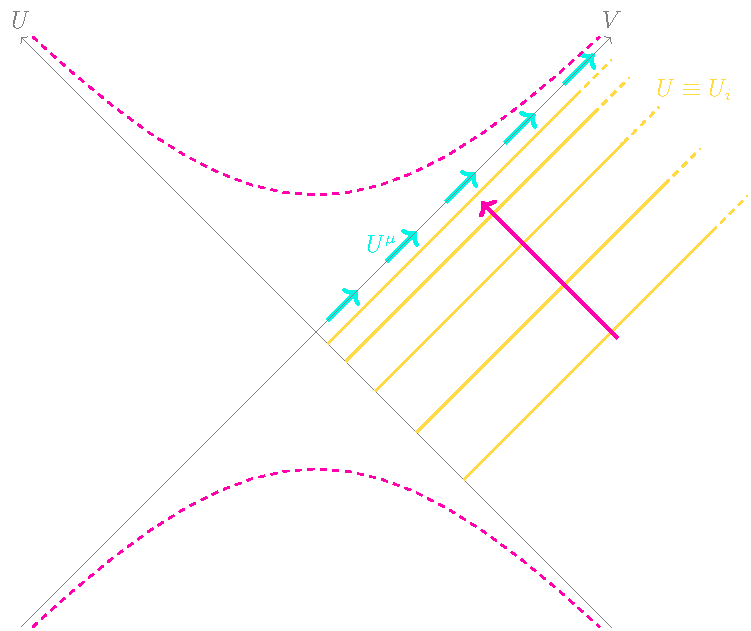
\includegraphics[scale=1.1]{Immagini/Kruskal-extension/Kruskal-extension.pdf}
    \caption{Penrose diagram of the maximally extended Schwarzschild solution. The cyclamen dashed line is the singularity, while the tuquoise arrows represent the vector field of null generators. When we take the limit \(U\rightarrow 0\) that finally leads us \eqref{eq:contraction-stress-tensor}, we choose to do it along the cyclamen solid arrow, where for each \(U_i\) we are considering the contraction with the field tangent to the null geodesic \(U \equiv U_i\), represented here by yellow solid lines.}
    \label{fig:Penrose-diagran-Kruskal-extension}
\end{figure}
Recall the identity
\[
UV = - \frac{r}{R_s} (1 - z) e^(\frac{r}{R_s}) \implies U^2 = \frac{(1 - z)^2}{z^2}  \frac{e^z}{V^2}
\]
and indeed
\begin{equation}
    \label{eq:contraction-nearly-done}
    \langle T^{\mu\nu}\rangle U_{\mu}U_{\nu} = 4e\frac{(1 - z)^2}{V^2}\left[\rho - 2f - \tau\right]. 
\end{equation}
Finally, we can substitute the expressions for \(\rho\), \(f\) and \(\tau\); according to Visser:
\begin{align*}
    \rho(z) &= -f_0 \frac{z^2}{(1 - z)^2} - F(z) \frac{z^2}{(1 - z)^2} + \text{reg}, \\
    \tau(z) &= f_0 \frac{z^2}{(1 - z)^2} + F(z) \frac{z^2}{(1 - z)^2} + \text{reg}, \\
    f(z) &= f_0 \frac{z^2}{(1 - z)^2},
\end{align*}
where we didn't bother writing terms regular on the horizion, as they get suppressed by the extra factor \((1 - z)^2\) in \(\eqref{eq:contraction-nearly-done}\). By recalling the definition of \(F(z)\) we can observe that near the horizion \(F(z) = O[(1 - z)^2]\), and hence \(F(z)\) also provides regular terms that will be suppressed for \(z \simeq 1\).

In the end we find
\begin{equation}
    \label{eq:contraction-stress-tensor}
    \langle T^{\mu\nu}\rangle U_{\mu}U_{\nu} =  -16f_0\frac{e}{V^2}
\end{equation}
The contraction becomes singular on the past horizion, at \(V = 0\), as expected, but it remains regular anywhere else on the future horizion, it is always negative (so we have everywhere a violation of the null energy condition), and its value goes as \(f_0 \propto M^{-4}\). 

Notice that these two last features only derive from the very minimal requirements of positive luminosity, and the matching with the expected well-known behaviour of the stress tensor in flat background (at spatial infinity). It is exactly the minimality of these requirements that provides such robustness to our result.

Finally, it is worth pointing out that this computation also shows explicitely that in the Schwarzschild solution the stress tensor observes the averaged condition:

\begin{equation}
    \label{eq:computation-averaged-contraction}
    \int_{V_0}^{+\infty} T_{\mu\nu}U^{\mu}U^{\nu} dV = - \frac{16ef_0}{V_0^2}.
\end{equation}
Speaking strictly about the Schwarzschild solution this bound would diverge because we would have \(V_0\rightarrow 0\), but this would correspond to integrating along the full future horizion on an eternal black hole spacetime, which physically corresponds to a black hole that Hawking-radiates for an infinite time: no surprise that we get a divergence!
For the Unruh vacuum state to be everywhere well defined instead, we must consider instead physically realistic spacetimes where the black hole forms for gravitational collapse at a finite time in the past, corresponding to a minimal value of \(V_{min} = V_0\). For such spacetimes we find that the integral in  \eqref{eq:computation-averaged-contraction} is negative but finite, and hence energy conditions such as the Sobolev conditions gain credibility.
Considerations of this sort had been made for \(2\) dimensional spacetimes already in \cite[]{ford1996averaged}, where however Ford and Roman rely on the analytical expansion of the stress tensor for the \(2\)-dimensional Unruh vacuum. They try to generalise the discussion to \(4\) dimensional spacetimes, claiming that equivalent bounds shall hold, (and anticipating they could be used to generalise Singularity theorems), but they don't manage to compute the contraction we derived in this appendix.

